\documentclass{article}
\usepackage{titling}
\usepackage{graphicx}
\usepackage{pgfgantt}
\usepackage{pdflscape}
\usepackage{hyperref}
\usepackage{animate}
\usepackage{movie15}
\usepackage[absolute,overlay]{textpos}
\usepackage{xspace}
\usepackage{subcaption}
\usepackage{listings}
\usepackage{amsmath}
\usepackage{caption}



\pretitle{
  \begin{center}
  \LARGE\bfseries
  
\includegraphics[width=0.2\textwidth]{image/logo.png} % Başlık önüne ekleyeceğiniz bir logo
  \vskip 1em
}
\title{Python ile Derin Öğrenme Kullanarak Otonom Bir Araba Oluşturmak}
\author{Ali Kağan Uyanık}
\date{Nisan 2024}


\begin{document}
\begin{titlingpage}
    \maketitle
    \begin{center}
        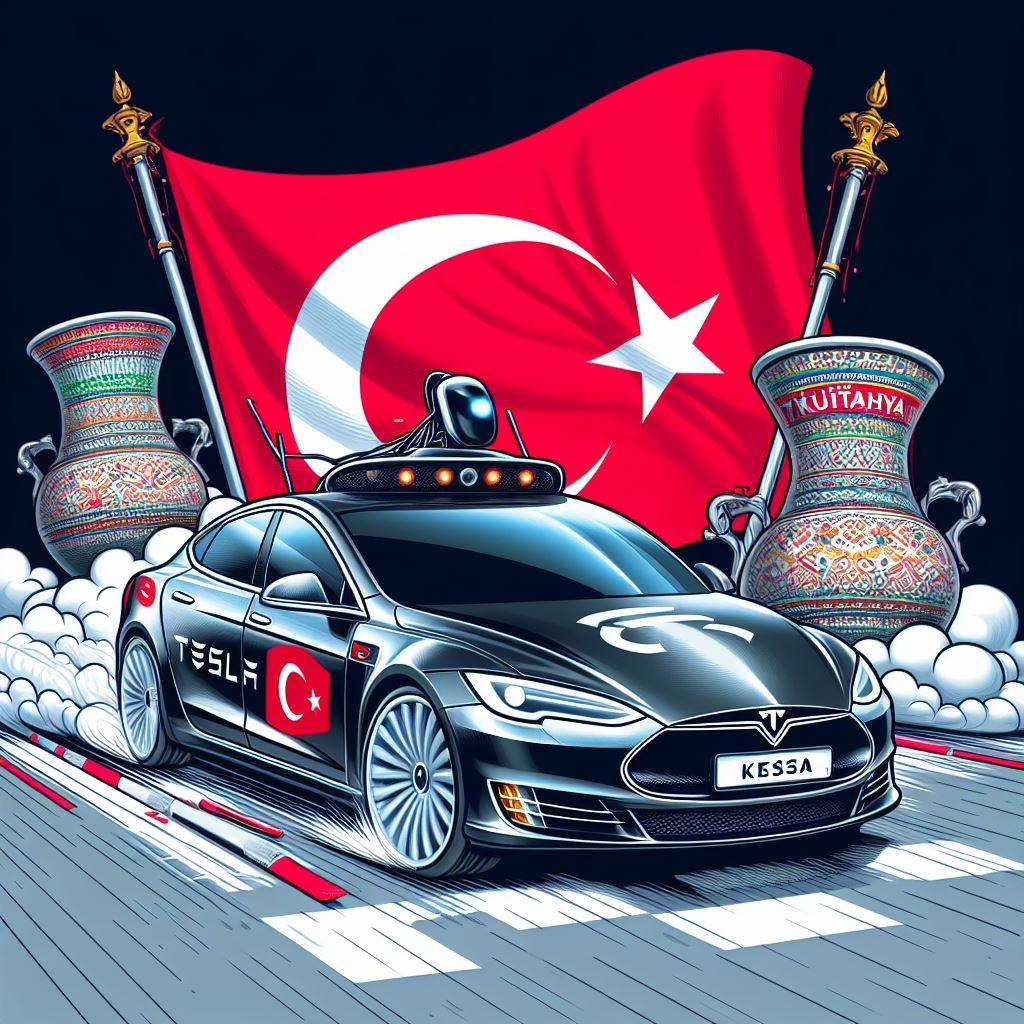
\includegraphics[width=0.6\textwidth]{image/keslakutahyada.jpg} % Araba resminin dosya adını belirtin
    \end{center}
    \vfill
    \rule{\textwidth}{0.5pt}
    \renewcommand{\abstractname}{Özet}
    \begin{abstract}
        \noindent Bu rapor, derin öğrenme tekniklerini anlamak ve bu tekniklerin otonom araç sistemlerindeki uygulamalarını göstermeyi hedeflemektedir.Projenin ilerleyen aşamalarında, bu tekniklerin bir simülasyon ortamına aktarılması planlanmaktadır.
    \end{abstract}
    \rule{\textwidth}{0.5pt}
    \vfill
\end{titlingpage}
\newpage
\section{Giriş}
\noindent Otomobilin kendisi kadar eski olan otonom sürüş hayali, yüksek derecede karmaşık bilgisayar sistemlerinin ve hassas kameraların ve sensörlerin icadından önce dahi var olmuştur. İnsanlar, gelecekteki araçların tamamen insan sürücüsünün etkisi olmadan çalışabileceği fikriyle büyülenmişlerdir.\\[5pt]
Sürüş neredeyse herhangi bir insanın kolayca yapabileceği bir aktivitedir. Ayrıca, sürüş sırasında gerçekleştirilmesi gereken çok az sayıda olası eylem vardır; bunlar genellikle hızlanma, fren yapma ve direksiyon kullanma ile sınırlıdır. Ancak, bu zorluğun beklenenden çok daha karmaşık olduğu ve bazı görsel veya bilişsel görevlerin bir bilgisayar için insan kadar kolay gerçekleştirilmediği hızla ortaya çıkar.Bu sorunlar ve bunları çözmek için olası yaklaşımlar, bu raporun ana odak noktasıdır.
\subsection{Otonom Sürüş Araçlarının Önemi}
Otonom araçlar, insan müdahalesi olmadan seyahat edebilen araçlardır. Bu teknolojinin öncelikli hedefi, trafik kazalarını azaltmak ve trafik verimliliğini artırmaktır. Sensörler ve yapay zeka kullanarak çevrelerindeki nesneleri algılayan otonom araçlar, trafikteki riskleri en aza indirmeyi amaçlar. Ayrıca, sürücülere daha fazla konfor ve güvenlik sağlarlar ve engelli bireylerin hareketliliğini artırabilirler. Ancak, bu teknolojinin benimsenmesi ve kullanımıyla ilgili teknik, etik ve yasal konular da dikkate alınmalıdır.\\[3pt]
\begin{figure}[h]
  \centering
  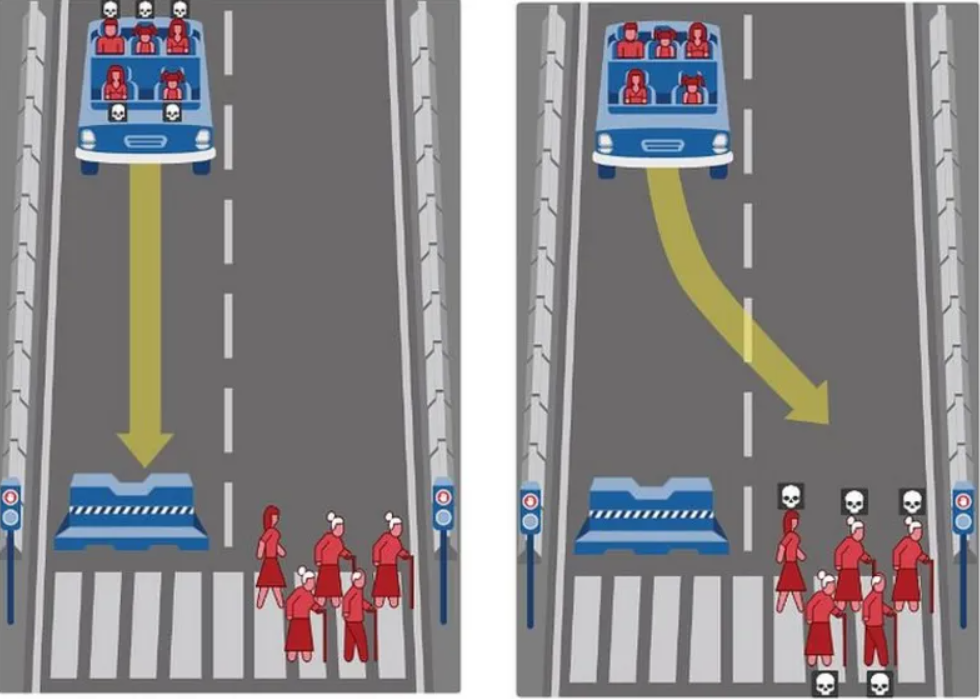
\includegraphics[width=0.9\textwidth]{image/Resim53.PNG} % Resim dosyasının adını ve uzantısını belirtin
  \caption{Mümkün olan ahlaki ikilemlerden biri \cite{Dilemma}}
  \label{fig:python16}  
\end{figure}
\newpage
\section{Otonom bir arabanın şerit çizgilerini belirlemek için OpenCV aracılığıyla Bilgisayarla Görme tekniklerini kullanması}
Bu kısmın amacı, bir resim veya videodaki şerit çizgilerini tanımlayabilen bir program geliştirmektir.İnsanlar araba kullanırken gözlerini kullanarak şerit çizgilerinin yerini belirleyebilirler, ancak araçlarımızın bu tür bir görsel algılama yeteneği yoktur. \\[5pt]
İşte bu noktada bilgisayarlı görme(computer vision) devreye giriyor, karmaşık algoritmalar aracılığıyla bilgisayarın görmesine yardımcı oluyor.


\begin{textblock*}{5cm}(17cm,1cm) % (17cm, -2cm) koordinatlarına bir text block oluşturulur
    
\includegraphics[width=2cm]{image/Resim17.png} % Resmin dosya adı ve boyutu
\end{textblock*}


\subsubsection{Grayscale Conversion(Gri Tonlamalı Dönüşüm)}
Kenar algılamanın amacı, görüntülerdeki nesnelerin sınırlarını tanımlamaktır. Temel olarak, bir görüntüde keskinliğin olduğu bölgeleri bulmaya çalışmak için kenar algılama kullanacağım.\\[1pt]

\noindent Bir görüntü bir matris, bir dizi olarak okunabilir.Bir piksel, görüntünün belirli bir yerindeki ışık yoğunluğunu içerir. Her piksel, 0 ile 255 arasında değişen sayısal bir değerle gösterilen yoğunluktur.\\[1pt]


\noindent Gradyan, bir dizi piksel üzerindeki parlaklıktaki değişikliktir.
Güçlü bir eğim, dik bir değişim kenarını gösterirken, küçük bir eğim, sığ bir değişimi temsil eder.

\begin{figure}[h]
  \centering
  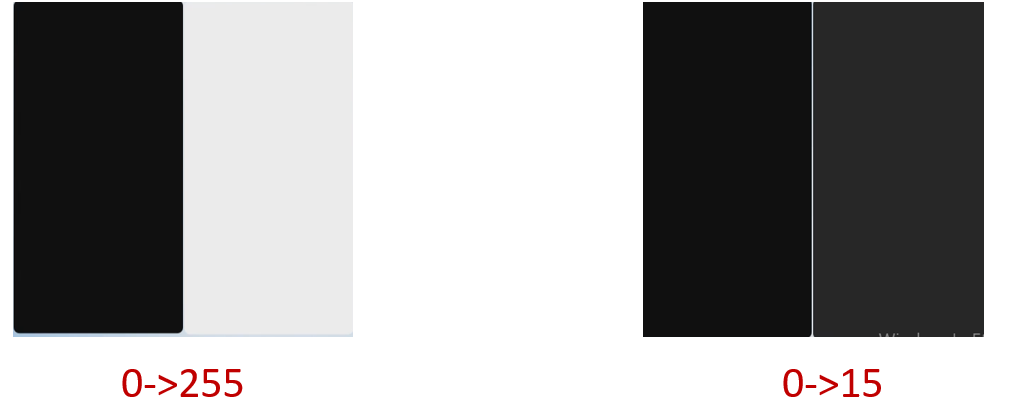
\includegraphics[width=1\textwidth]{image/Ekran Alıntısı4.PNG} % Resim dosyasının adını ve uzantısını belirtin
  \caption{Strong Gradient ve Small Gradient}
  \label{fig:python16}  
\end{figure}
\newpage
\begin{textblock*}{5cm}(17cm,1cm) % (17cm, -2cm) koordinatlarına bir text block oluşturulur
    
\includegraphics[width=2cm]{image/Resim17.png} % Resmin dosya adı ve boyutu
\end{textblock*}
\noindent Bir kenar yoğunluk farkıyla tanımlandığından bu görüntümüzdeki kenarları tanımlamamıza yardımcı olur.
\begin{figure}[h]
  \centering
  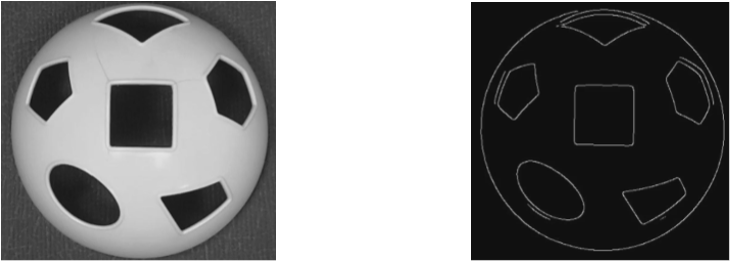
\includegraphics[width=1\textwidth]{image/Ekran Alıntısı5.PNG} % Resim dosyasının adını ve uzantısını belirtin
  \caption{Orijinal ve Gradient Görüntü}\cite{mordvintsev2014opencv}
  \label{fig:python17}  
\end{figure}
\subsubsection{Neden Görseli Gri Tonlamaya Dönüştürmeliyim?}
Görüntüler piksellerden oluşur.\\[2pt]
Üç kanallı renkli bir görüntüde kırmızı, yeşil ve mavi kanallar bulunur.\\[2pt]
Gri tonlamalı bir görüntüde her pikselde yalnızca bir kanal bulunur ve yalnızca bir yoğunluk değeri vardır.\\[2pt]
Renk bilgisinin olmaması daha az veri kullanımı ve daha basit işleme süreçleri anlamına gelir.\\[2pt]
\begin{figure}[h]
  \centering
  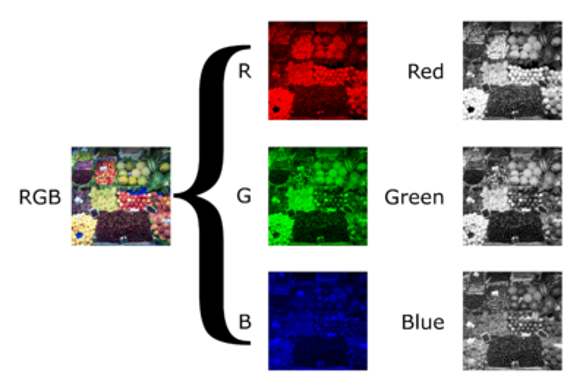
\includegraphics[width=0.8\textwidth]{image/Resim20.png} % Resim dosyasının adını ve uzantısını belirtin
  \label{fig:python18} 
  \caption{Gri tonlama \cite{mordvintsev2014opencv}}
\end{figure}
\newpage
\begin{textblock*}{5cm}(17cm,1cm) % (17cm, -2cm) koordinatlarına bir text block oluşturulur
    
\includegraphics[width=2cm]{image/Resim17.png} % Resmin dosya adı ve boyutu
\end{textblock*}
\begin{figure}[h]
  \centering
  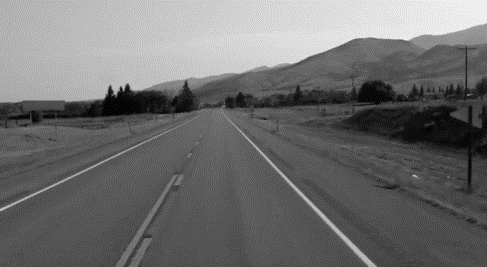
\includegraphics[width=0.9\textwidth]{image/Resim21.png} % Resim dosyasının adını ve uzantısını belirtin
  \caption{Gri Tonlama Uygulanan Görsel}
  \label{fig:python19}  
\end{figure}
\subsubsection{Gauss bulanıklığı}
Görüntü gürültüsü sahte kenarlar oluşturabilir ve sonuçta kenar algılamayı etkileyebilir.\\[2pt]
Artık gürültüyü azaltmalı ve kenarları tespit ederken görüntümüzü yumuşatmalıyız.
\begin{figure}[h]
  \centering
  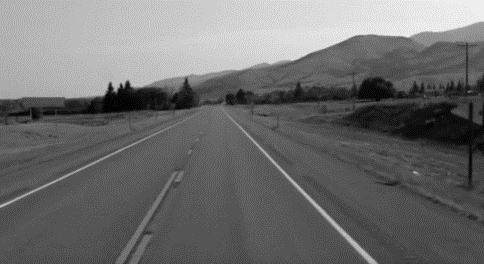
\includegraphics[width=0.9\textwidth]{image/Resim22.png} % Resim dosyasının adını ve uzantısını belirtin
  \caption{Gauss Bulanıklığı Uygulanan Görsel}
  \label{fig:python20}  
\end{figure}
\newpage
\begin{textblock*}{5cm}(17cm,1cm) % (17cm, -2cm) koordinatlarına bir text block oluşturulur
    
\includegraphics[width=2cm]{image/Resim17.png} % Resmin dosya adı ve boyutu
\end{textblock*}
\subsubsection{Canny Kenar Tespiti (Edge Detection)}
Bu metodu,görüntüdeki kenarları belirlemek için kullanacağım.\\[2pt]
Bir kenar, görüntüde yoğunlukta keskin bir değişikliğin olduğu bir bölgeye karşılık gelir.\\[2pt]
Canny fonksiyonunun bizim için yapacağı şey, fonksiyonumuzun hem X hem de Y yönünde bir türevini gerçekleştirmektir, böylece bitişik piksellere göre yoğunluktaki değişim ölçülür.\\[2pt]
Küçük bir türev yoğunluktaki küçük bir değişikliktir, büyük bir türev ise büyük bir değişikliktir.\\[2pt]
Gradyan üst eşikten büyükse kenar pikseli olarak kabul edilir. Alt eşiğin altında ise reddedilir.\\[5pt]
\begin{figure}[h]
  \centering
  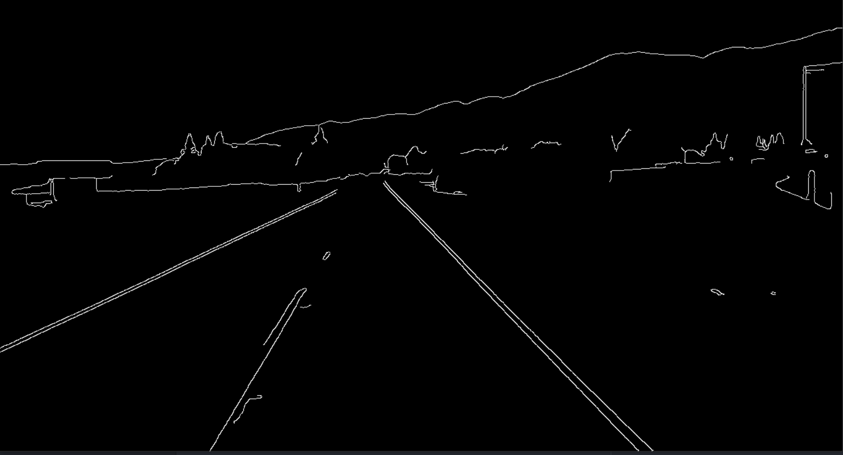
\includegraphics[width=0.9\textwidth]{image/Resim23.png} % Resim dosyasının adını ve uzantısını belirtin
  \caption{Canny Metodu Uygulanan Görsel}
  \label{fig:python21}  
\end{figure}
\subsubsection{İlgi Bölgesi}
Şerit çizgilerini nasıl tanımlayabileceğimize odaklanmadan önce yapmamız gereken imajımızda gideceğimiz ilgi alanını belirlemektir. 
\newpage
\begin{textblock*}{5cm}(17cm,1cm) % (17cm, -2cm) koordinatlarına bir text block oluşturulur
    
\includegraphics[width=2cm]{image/Resim17.png} % Resmin dosya adı ve boyutu
\end{textblock*}
\begin{figure}[h]
  \centering
  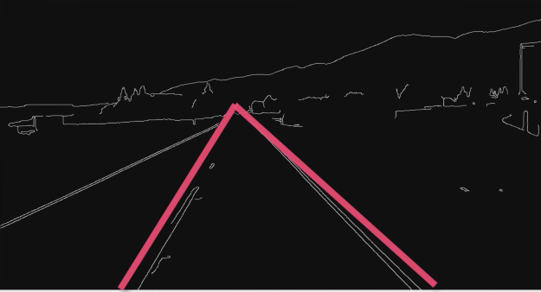
\includegraphics[width=0.9\textwidth]{image/Resim24.png} % Resim dosyasının adını ve uzantısını belirtin
  \caption{İzole edilecek bölge}
  \label{fig:python22}  
\end{figure}
\noindent Görüş alanımızın kapsamını ilgi alanına göre sınırlayacağız.\\[5pt]
Bölgeyi nasıl izole edeceğimi daha iyi açıklığa kavuşturmak için Matplotlib kütüphanesini kullanacağım. Anaconda dağıtımının içinde geldiği için onu projede içe aktarmalıyız.\\[5pt]

\begin{figure}[h]
  \centering
  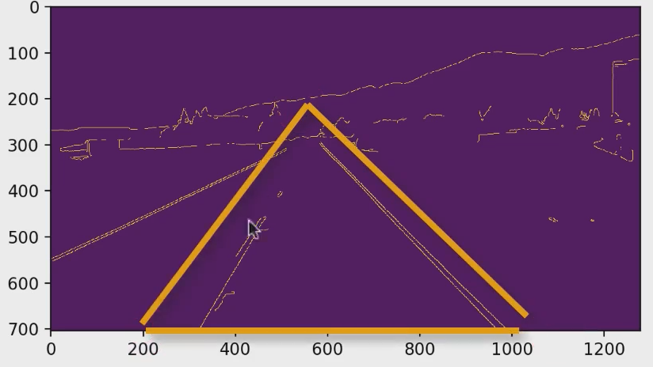
\includegraphics[width=0.9\textwidth]{image/Resim25.png} % Resim dosyasının adını ve uzantısını belirtin
  \caption{Görüş alanı}
  \label{fig:python23}  
\end{figure}

\newpage
\begin{textblock*}{5cm}(17cm,1cm) % (17cm, -2cm) koordinatlarına bir text block oluşturulur
    
\includegraphics[width=2cm]{image/Resim17.png} % Resmin dosya adı ve boyutu
\end{textblock*}
\noindent Şimdi yapacağımız şey ilgilenilen bölgenin fonksiyonunu tanımlamak.\\[5pt]
Görüş alanımızın kapalı bölgesini döndürecek ve kapalı bölgenin üçgen olduğunu hatırlatacak şekilde olmalı.

\begin{figure}[h]
  \centering
  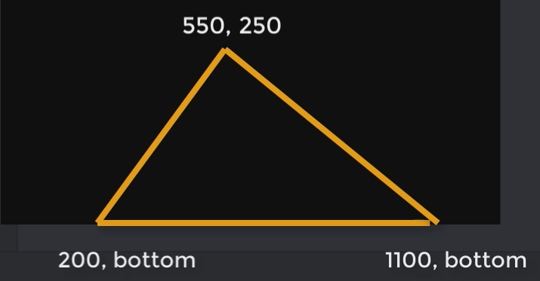
\includegraphics[width=0.9\textwidth]{image/Resim26.png} % Resim dosyasının adını ve uzantısını belirtin
  \caption{Görüş alanı koordinatları}
  \label{fig:python24}  
\end{figure}
\noindent Bu koordinatlara göre bir maske oluşturuldu.\\[1pt]
İşte bu oluşturduğum maske.\\[5pt]

\begin{figure}[h]
  \centering
  
\includegraphics[width=0.9\textwidth]{image/Resim27.png} % Resim dosyasının adını ve uzantısını belirtin
  \caption{Bu görüntü,canny görüntüsünü maskelemek için kullanılacaktır.}
  \label{fig:python25}  
\end{figure}
\newpage
\begin{textblock*}{5cm}(17cm,1cm) % (17cm, -2cm) koordinatlarına bir text block oluşturulur
    
\includegraphics[width=2cm]{image/Resim17.png} % Resmin dosya adı ve boyutu
\end{textblock*}
\begin{figure}[h]
  \centering
  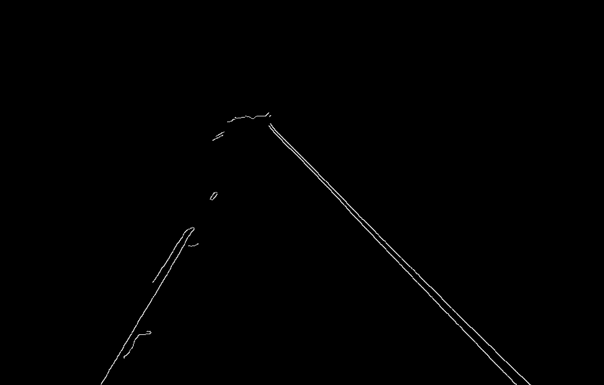
\includegraphics[width=0.9\textwidth]{image/Resim28.png} % Resim dosyasının adını ve uzantısını belirtin
  \caption{İlgilenilen bölge izole edildi ve diğer her şeyi maskelendi.}
  \label{fig:python26}  
\end{figure}

\subsubsection{Hough Dönüşümü}
Hough Dönüşümü, bir görüntüdeki düz çizgileri algılayan bir tekniktir.\\[5pt]
Hough dönüşümü, bir görüntüdeki doğru hattı temsil eden parametrelere sahip olasılık yoğunluk alanını (Hough uzayı) oluşturur. Bu, her bir pikselin bir hattaki olası konumları için bir oylama sürecini içerir.

\begin{figure}[h]
  \centering
  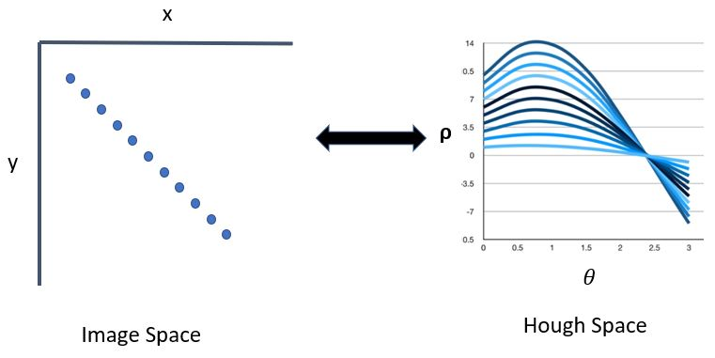
\includegraphics[width=0.9\textwidth]{image/Resim29.png} % Resim dosyasının adını ve uzantısını belirtin
  \caption{Görüntü alanından Hough alanına\cite{ranjan2020applied}}
  \label{fig:python27}  
\end{figure}
\newpage
\begin{textblock*}{5cm}(17cm,1cm) % (17cm, -2cm) koordinatlarına bir text block oluşturulur
    
\includegraphics[width=2cm]{image/Resim17.png} % Resmin dosya adı ve boyutu
\end{textblock*}
\begin{figure}[h]
  \centering
  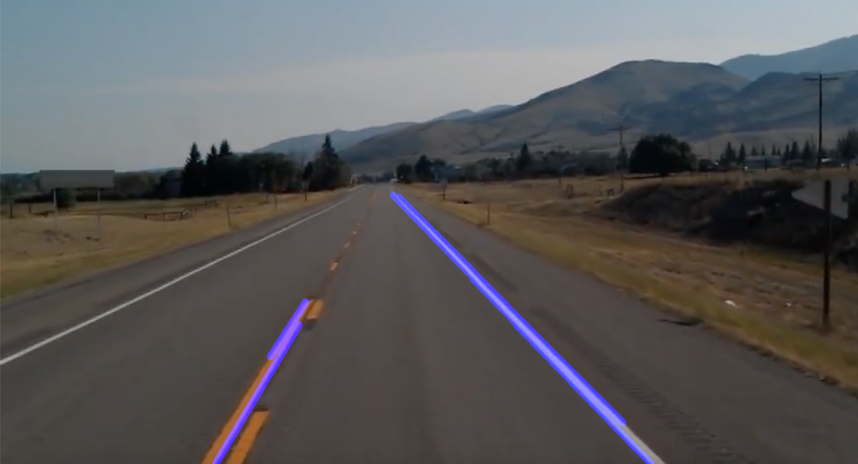
\includegraphics[width=0.8\textwidth]{image/Resim30.png} % Resim dosyasının adını ve uzantısını belirtin
  \caption{En yüksek oylara sahip noktalardan elde edilen parametreler kullanılarak, orijinal görüntü üzerine çizgi çizdirildi.Bu çizgiler şerit çizgilerini temsil etmektedir.}
  \label{fig:python28}  
\end{figure}

\subsubsection{Optimize etme}
Optimizasyonu gerçekleştirmek için, algılanan çizgilerin eğimlerini ve y-kesişimlerini ortalayarak tek bir çizgi oluşturma hedeflenmekteddir. Bu, daha net ve düzgün bir görüntü elde etmek için birden çok çizgi yerine her iki şerit için sadece bir çizgi kullanmamızı sağlayacak. İlk adım olarak, her iki şerit için ayrı ayrı ortalama eğim ve y-kesişimini hesaplayacağız. Ardından, bu ortalama değerleri kullanarak her iki şerit için tek bir çizgi oluşturacağız. Bu optimize edilmiş yaklaşım, daha az karmaşıklıkla daha etkili bir sonuç elde etmemizi sağlayacak.\\[5pt]

\begin{figure}[h]
  \centering
  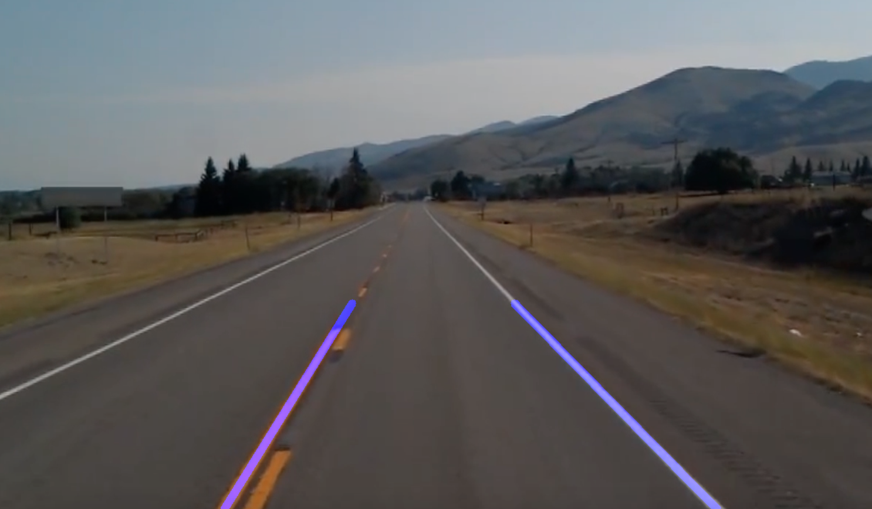
\includegraphics[width=0.8\textwidth]{image/Resim31.png} % Resim dosyasının adını ve uzantısını belirtin
  \caption{Son hal}
  \label{fig:python29}  
\end{figure}
\newpage
\begin{textblock*}{5cm}(17cm,1cm) % (17cm, -2cm) koordinatlarına bir text block oluşturulur
    
\includegraphics[width=2cm]{image/Resim17.png} % Resmin dosya adı ve boyutu
\end{textblock*}
\subsubsection{Videoda Şerit Bulma Çalışması}
Resimdeki şerit çizgilerinin belirlenmesi için geliştirilen algoritma, aynı yöntem ile video formatında da uygulanmıştır. Video çerçeveleri üzerinde algoritma tekrar tekrar uygulanmış ve sonuçlar ekranda gösterilmiştir. Ayrıca, videonun kapatılması için bir klavye tuşuna basma işlevselliği eklenmiştir.

\begin{textblock*}{5cm}(17cm,1cm) % (17cm, -2cm) koordinatlarına bir text block oluşturulur
    
\includegraphics[width=2cm]{image/Resim17.png} % Resmin dosya adı ve boyutu
\end{textblock*}

\section{Perceptron(Algılayıcı)}
Bir otonom aracın ilk yapacağı iş çevresini algılamaktır. 
\subsection{Makine Öğrenmesi}
Makine öğrenimi, deneyime dayalı olarak zaman içinde öğrenen hesaplamalı sistemler oluşturma kavramıdır.
Makine öğrenmesi, kısaca verilerle öğrenme becerisidir.
Öğrenme, öğrenci ile çevre arasında gerçekleşir. Bu bağlamda denetimli ve denetimsiz öğrenmeyi birbirinden ayırmak önemlidir.
\subsection{Denetimli Öğrenme(Supervised Learning)}
Denetimli öğrenme, modelin eğitim sürecinde giriş verileri ve gerçek çıktıları (hedefler) kullanır. Model, bu verileri kullanarak girdilerle çıktılar arasındaki ilişkiyi öğrenir ve daha sonra yeni, daha önce görmediği girdilerle karşılaştığında doğru çıktıları tahmin edebilir.
\subsection{Denetimsiz Öğrenme(Unsupervised Learning)}
Denetimsiz öğrenme, bir modelin girdi verileri arasındaki doğal yapıları veya desenleri belirlemeye çalıştığı bir süreci ifade eder, ancak bu desenlerin ne olduğu önceden bilinmez veya belirtilmemiştir.

\newpage
\begin{textblock*}{5cm}(17cm,1cm) % (17cm, -2cm) koordinatlarına bir text block oluşturulur
    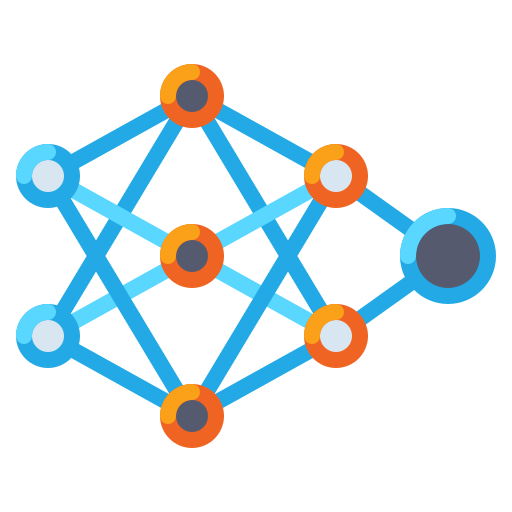
\includegraphics[width=2cm]{image/sinir.png} % Resmin dosya adı ve boyutu
\end{textblock*}
\subsection{Doğrusal Regresyon}
Denetimli öğrenmenin bir biçimidir.\\[5pt]
Bir model, girdiye dayalı olarak sürekli bir çıktıyı tahmin etmek için eğitilir. Örneğin, bir evin fiyatını tahmin etmek için evin özelliklerini (odaların sayısı, konumu, vb.) kullanmak gibi.
\begin{figure}[h]
  \centering
  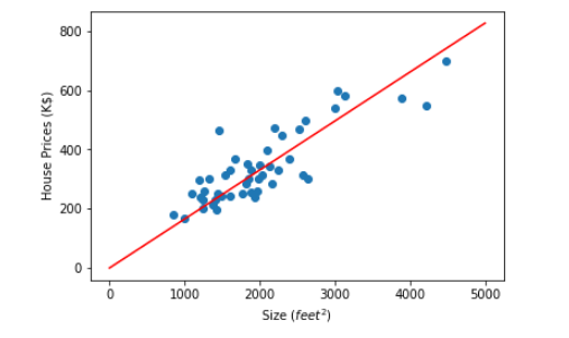
\includegraphics[width=0.7\textwidth]{image/Resim35.png} % Resim dosyasının adını ve uzantısını belirtin
  \caption{Örnek lineer regresyon modeli \cite{pardoe2020applied}}
  \label{fig:python33}  
\end{figure}
\subsection{Sınıflandırma}
Belirli bir girdiye dayalı olarak belirli bir çıktı sınıfını (kategori) tahmin etmeyi amaçlar.\\[5pt]
Sürücüsüz otomobillerde sınıflandırma problemlerini çözmek son derece önemlidir. Bu, yoldan geçen nesnelerin araba mı, yaya mı, bisiklet mi olduğunu sınıflandırmak ve hatta farklı trafik işaretlerini tanımlamak için kullanılabilir.\\[2pt]
\begin{figure}[h]
  \centering
  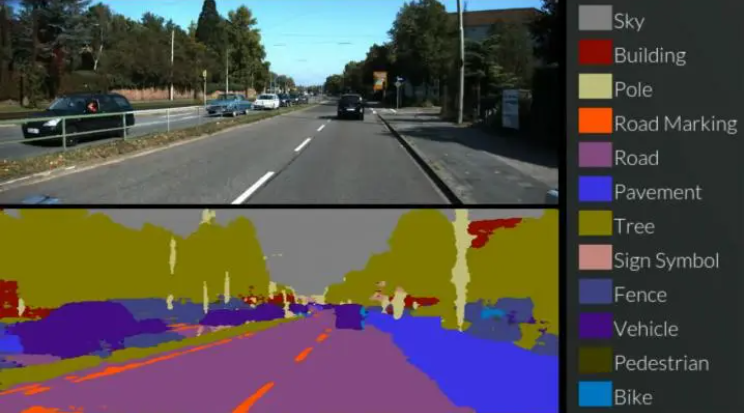
\includegraphics[width=0.7\textwidth]{image/Resim36.png} % Resim dosyasının adını ve uzantısını belirtin
  \caption{SegNet(Semantic Segmentation)\cite{deepika2017obstacle}}
  \label{fig:python34}  
\end{figure}
\newpage
\begin{textblock*}{5cm}(17cm,1cm) % (17cm, -2cm) koordinatlarına bir text block oluşturulur
    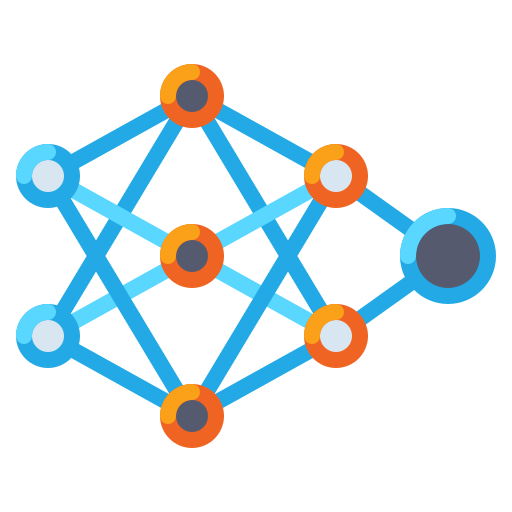
\includegraphics[width=2cm]{image/sinir.png} % Resmin dosya adı ve boyutu
\end{textblock*}

\subsection{Lojistik Regresyon ile Sınıflandırma Projesi}
Bu proje, temel bir lojistik regresyon modelini oluşturmak için Python ve numpy kütüphanelerini kullanmaktadır.Kod,iki farklı bölgeye ayrılmış bir veri setini içermektedir:üst bölge (kırmızı noktalar) ve alt bölge (mavi noktalar).Amacımız, bu iki bölge arasındaki sınırlayıcı çizgiyi belirlemektir. Bu çizgiyi belirlemek için, gradient inişi adı verilen bir optimizasyon algoritması kullanılmıştır.Gradient inişi, bir hatanın minimize edilmesinde kullanılan bir yöntemdir. Bu projede, çapraz entropi hatası kullanılarak modelin performansı değerlendirilmiştir.Model, bu hata fonksiyonunun minimum değerini bulmaya çalışarak çizgi parametrelerini günceller.

\noindent Sonuçlar, veri setindeki noktaların sınıflandırılmasında kullanılan çizgiyi göstermektedir. Grafik üzerindeki çizgi, lojistik regresyon modelinin bulduğu sınırlayıcı çizgiyi temsil eder.Bu çizgi, veri noktalarını iyi bir şekilde ayırarak sınıflandırma yapmaktadır.

\noindent Bu proje, temel bir lojistik regresyon modelinin nasıl oluşturulacağını ve optimize edileceğini anlamak için bir başlangıç noktası olarak kullanılabilir.
\begin{figure}[h]
    \centering
    \begin{subfigure}{0.5\textwidth}
        \centering
        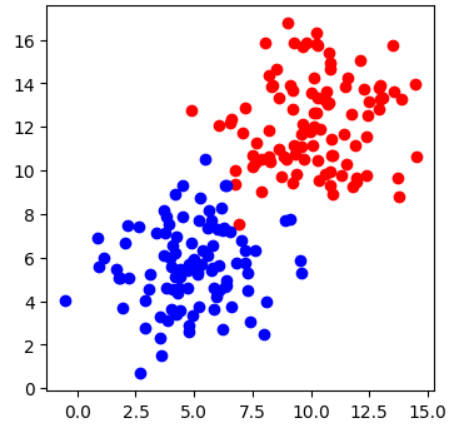
\includegraphics[width=1\linewidth]{image/Resim54.PNG}
        \caption{Dağılım grafiği}
        \label{fig:resim1}
    \end{subfigure}%
    \begin{subfigure}{0.5\textwidth}
        \centering
        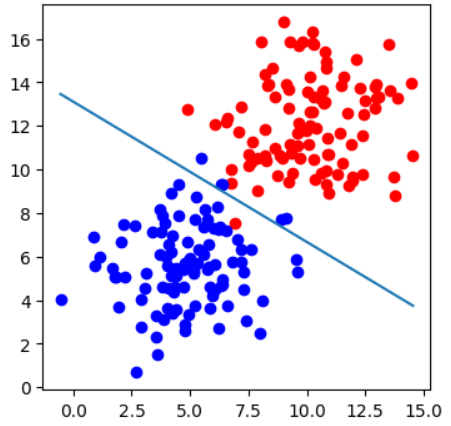
\includegraphics[width=1\linewidth]{image/Resim55.PNG}
        \caption{Sonuç}
        \label{fig:resim2}
    \end{subfigure}
    \caption{Proje çıktıları}
    \label{fig:iki_resim}
\end{figure}

\subsection{Sinir Ağları}
İnsan gibi düşünen bir makine yapılabilir mi sorusundan doğmuştur.İnsanın öğrenme şeklini taklit eder.\\[5pt]
Beyin, milyarlarca sinir hücresi veya nöron aracılığıyla bilgiyi işler. Sinir ağları da bu doğal süreçten esinlenerek bilgiyi işlemek, desenleri tanımak, tahmin yapmak ve karar vermek için kullanılır.\\[5pt]
Bu projede, bir arabanın o anda pistin hangi bölümünde olduğuna göre kendi başına gidebileceği direksiyon açılarını tahmin etmek için bir sinir ağından faydalanacağım.\\[5pt]
Nörona sağdan soldan bilgiler akar, bu akan bilgilere göre nöron bir karar verir ve iletim yapar veya yapmaz.

\begin{textblock*}{5cm}(17cm,1cm) % (17cm, -2cm) koordinatlarına bir text block oluşturulur
    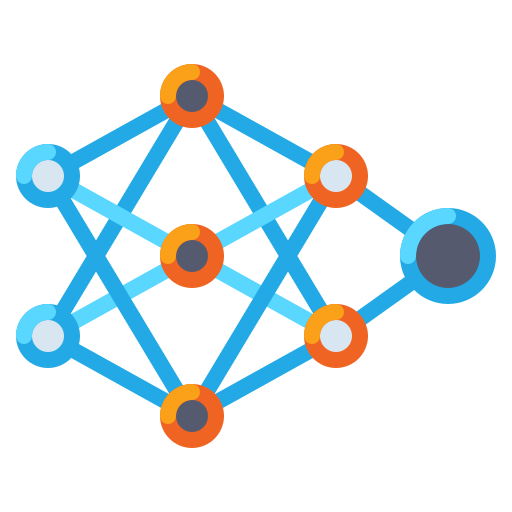
\includegraphics[width=2cm]{image/sinir.png} % Resmin dosya adı ve boyutu
\end{textblock*}
\begin{figure}[h]
  \centering
  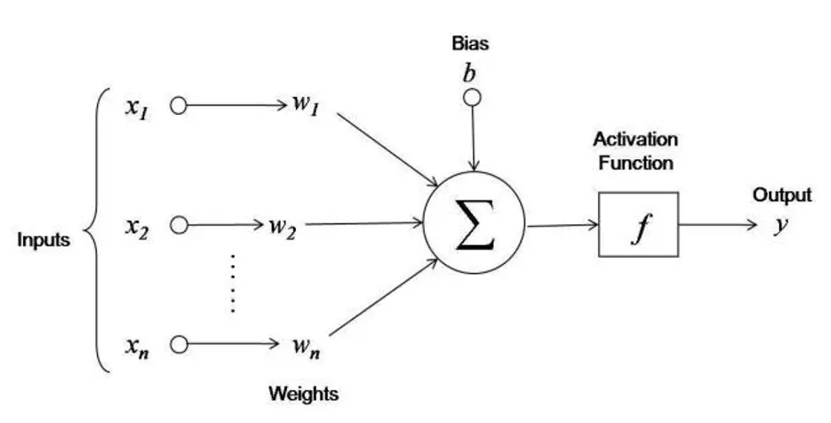
\includegraphics[width=0.9\textwidth]{image/Resim38.png} % Resim dosyasının adını ve uzantısını belirtin
  \caption{Sinir ağı \cite{sze2017efficient}}
  \label{fig:python36}  
\end{figure}
\noindent Basit bir sinir ağı yapısına baktığımızda(single layer),duyargalar ve nöronlar arasındaki çizgilerin hepsinin bir ağırlık değeri vardır.Bir nörona akan verileri topladığımızda, 3 sensörden bilgi akıyor, her biri farklı bir ağırlık değeri ile çarpılır ve bu değerler toplanır.Toplam değer eşik değeri(threshold value) geçerse sinyal ateşlenir.\\[5pt]
Sinir ağlarında aktivasyon fonksiyonu, bir sinir hücresinin çıktısını belirlemek için kullanılan matematiksel bir işlemdir.


\section{Derin Sinir Ağları}
Derin sinir ağları, sürücüsüz araçların önemli bir parçasıdır. Yapay zeka ve sinir ağları kullanarak, araç, dinamik bir ortama tepki vermek için gerçek zamanlı kararlar alabilir. Derin sinir ağları kullanarak araç, kendi sensör verilerini kullanarak dünyada gezinebilir. Deneyim yoluyla öğrenerek, araç belirli koşulları tanımak ve kararlar almak için eğitilebilir.\\[5pt]
Araç öğrenme süreci için, belirli bir görev için ayrılmış bir sinir ağı kümesi son derece önemlidir. Örneğin, bir sinir ağı seti, sokak levhalarını okumak için veya insanları arka plandan tanımak için olabilir. Tüm zorluklar önceden tahmin edilmeli ve belirli bir görev için bir sinir ağı kümesi belirlenmelidir.\\[5pt]
Derin sinir ağları, giriş ve çıkış katmanları arasında birden çok katmana sahiptir. Bu tür bir mimari, doğrusal olmayan ilişkilere sahip bilgileri yorumlamada anahtardır. Gerçek zamanlı sürüş bilgisi genellikle doğrusal bir ilişkiye sahip değildir. Bilgi, çıkışı hesaplamak için katmanlar arasında hareket ederek yorumlanır.\\[4pt]
Otonom araçlar için kullanılan derin öğrenme ağları genellikle ileri beslemeli; veri geri dönüş yapmadan girişten çıkışa akar. Algoritma, belirli parametreleri daha etkili hale getirmek için ağırlıklar atar.Ardından,doğru yorumu manipülasyonuna dayanarak belirler.

\begin{textblock*}{5cm}(17cm,1cm) % (17cm, -2cm) koordinatlarına bir text block oluşturulur
    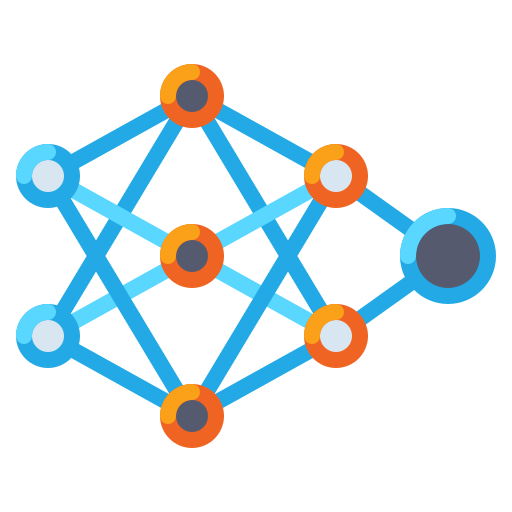
\includegraphics[width=2cm]{image/sinir.png} % Resmin dosya adı ve boyutu
\end{textblock*}
\subsection{Multi-Layer Perceptrons (MLP)}
Çok Katmanlı Algılayıcılar (MLP) , yapay sinir ağlarının bir türüdür ve giriş katmanı, en az bir gizli katman (ara katman) ve bir çıkış katmanından oluşur. Her bir katman, birbirine bağlı nöronlardan oluşur.MLP’ler ileri beslemeli sinir ağlarıdır.\\[4pt]
\begin{figure}[htbp]
    \centering
    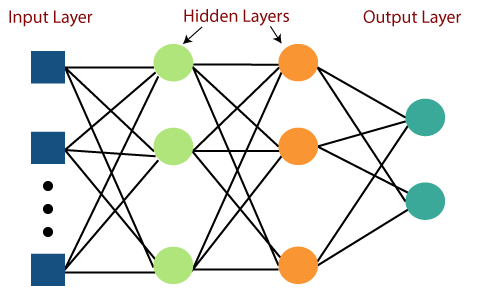
\includegraphics[width=0.9\textwidth]{image/Resim39.png}
    \caption{Multi-Layer Perceptron\cite{HiddenLayer}}
    \label{fig:python37}
    \vspace{0.2cm} % İstenirse biraz boşluk ekleyebilirsiniz
\end{figure}
\subsection{Yapay Sinir Ağı ile Sınıflandırma ve Tahmin Projesi}
Projede, bir yapay sinir ağı modeli kullanılarak bir sınıflandırma problemi çözülmüştür. Model, iki giriş özelliğine sahip veri noktalarını alır ve bunları iki sınıfa ayırmak için eğitilir. Model, ardından bu veri noktalarını ayıran karar sınırını öğrenir.\\[2pt]
İlk adımda, yapay sinir ağı modeli tanımlanır. Model, giriş katmanı, gizli katman ve çıkış katmanından oluşur. Giriş katmanı iki giriş özelliğini alırken, çıkış katmanı bir sınıf tahmini sağlar. Modelin eğitimi için gerekli olan optimizasyon ve kayıp fonksiyonları belirlenir.\\[2pt]
\newpage
\begin{textblock*}{5cm}(17cm,1cm) % (17cm, -2cm) koordinatlarına bir text block oluşturulur
    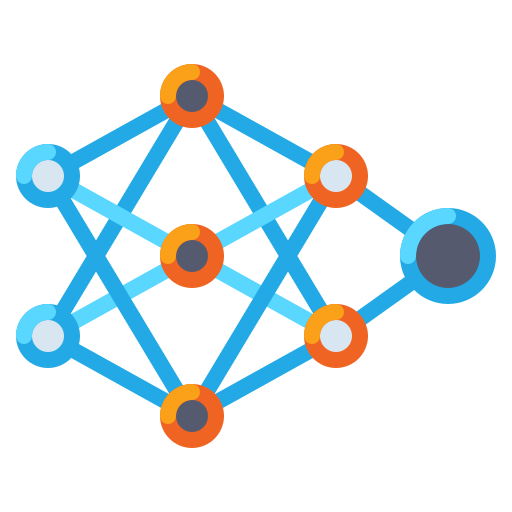
\includegraphics[width=2cm]{image/sinir.png} % Resmin dosya adı ve boyutu
\end{textblock*}
\noindent Daha sonra, model veri noktalarıyla eğitilir.Eğitim, veri noktalarının belirli bir batch boyutunda ve belirli bir epoch sayısında model tarafından işlenmesini içerir.Eğitim sırasında modelin başarısını ölçmek için doğruluk metriği kullanılır.\\[2pt]
Eğitim tamamlandıktan sonra, modelin karar sınırı çizilir. Bu, modelin öğrendiği sınıflandırma kararlarını görselleştirmeye olanak tanır. Ayrıca, belirli bir noktanın model tarafından tahmin edilmesi ve bu tahminin görselleştirilmesi sağlanır.\\[2pt]
Bu proje, yapay sinir ağlarının sınıflandırma problemlerini nasıl çözebileceğini ve bu modellerin nasıl görselleştirilebileceğini göstermektedir. Yapay sinir ağları, geniş bir uygulama yelpazesine sahip olan güçlü bir makine öğrenimi tekniğidir.

\begin{figure}[h]
  \centering
  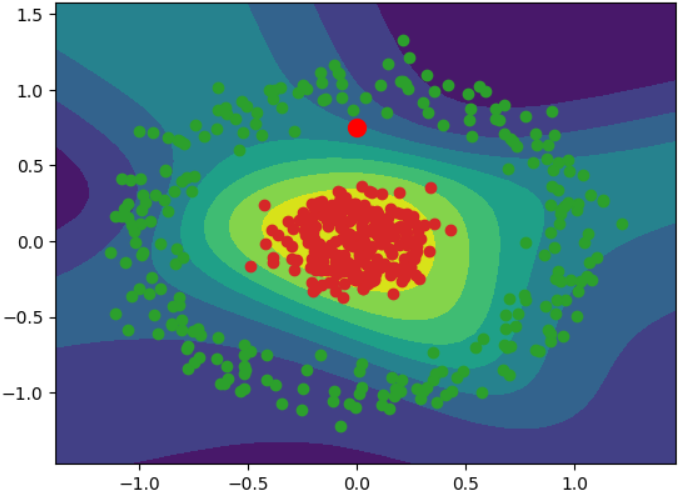
\includegraphics[width=1\textwidth]{image/Resim56.PNG} % Resim dosyasının adını ve uzantısını belirtin
\caption{Tahminin görselleştirilmesi}
  \label{fig:cnn}  
\end{figure}



\section{Hafta7: Evrişimli Sinir Ağları(CNN)}
Görüntülerin işlenmesinde ve özellikle otonom sürüş gibi alanlarda kullanılan evrişimli sinir ağları (ConvNets/CNN'ler), yapay zeka dünyasında büyük bir öneme sahiptir. Ancak, geleneksel çok katmanlı algılayıcılar, yüksek çözünürlüklü girdilerle başa çıkmakta zorlanır. Bir megapiksel çözünürlüğe sahip bir görüntü, milyonlarca bağlantı ve ağırlık içerir. Bu da ağın öğrenmesini zorlaştırır ve çok fazla bellek gerektirir.\\[2pt]
\newpage
\begin{textblock*}{5cm}(17cm,1cm) % (17cm, -2cm) koordinatlarına bir text block oluşturulur
    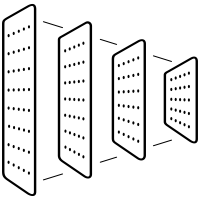
\includegraphics[width=2cm]{image/Resim45.png} % Resmin dosya adı ve boyutu
\end{textblock*}

\noindent ConvNet'lerin temel amacı, bu sorunu çözmek için geliştirilmiştir. Bu ağlar, yalnızca girdi verilerindeki belirli alanlarla etkileşime girerler ve ağırlıkları paylaşarak parametre sayısını azaltırlar. Yani, aynı özelliklere sahip olan pikseller arasındaki ilişkileri değerlendirirler ve bu özellikleri farklı alanlarda tekrar tekrar kullanırlar. Bu da daha az parametre kullanarak daha etkili bir şekilde öğrenmeyi sağlar.\\[2pt]

\noindent Özetle, ConvNet'ler, yüksek boyutlu girdi verilerini işlemek için optimize edilmiş ve daha az bellek ve hesaplama gücü gerektiren bir yapıya sahiptir. Bu da onları görüntü işleme, nesne tanıma ve otonom sürüş gibi uygulamalarda vazgeçilmez bir araç haline getirir
.
\subsection{Ağ Mimarisi}
CNN'ler, veriyi genişlik, yükseklik ve derinlik olmak üzere 3 boyutta temsil ederler.Bu, evrişimler, doğrusal olmayan fonksiyonlar ve pooling işlemlerinden oluşur. Sınıflandırma amaçları için tam bağlantılı bir katman ve bir softmax aktivasyon fonksiyonu eklenir. 


\subsection{Evrişimler}
Bu ağların ana parçaları, evrişim işlemleridir.Bu işlemler, özellik haritaları oluşturmak için çekirdekler veya filtreler kullanır.Evrişim çekirdeği, girdi matrisi üzerinde hareket eder ve girdiyi temel özelliklerine (özellik haritaları) indirgeyen bir evrişim işlemi uygular. Eğitim sırasında, ağ verilen problemi çözmek için hangi özelliklerin önemli olduğunu belirler. Örneğin, bir görüntüyü belirli bir kategoriye sınıflandırmak için hangi özelliklerin önemli olduğunu öğrenir.

\subsection{Evrişimsel Sinir Ağlarının Yapısı}
İşlevselliği elde etmek için, Cnn görüntüyü çeşitli katmanlarla işler. 
\subsubsection{Evrişimli Katman (Convolutional Layer)}
Bu katman, girdi verisindeki özellikleri belirlemek için kullanılır. Örneğin, bir görüntüdeki kenarları veya desenleri bulmak gibi. Evrişimli katman, özellik haritalarını oluşturmak için giriş verisi üzerinde filtreler uygular.
\subsubsection{Doğrusal Olmayanlık Katmanı (Non-Linearity Layer)}
 Bu katman, ağa doğrusal olmayanlık ekler. Bu, ağın daha karmaşık ilişkileri öğrenmesine olanak tanır. Genellikle ReLU (Rectified Linear Unit) veya sigmoid gibi aktivasyon fonksiyonları kullanılır.
\newpage
\begin{textblock*}{5cm}(17cm,1cm) % (17cm, -2cm) koordinatlarına bir text block oluşturulur
    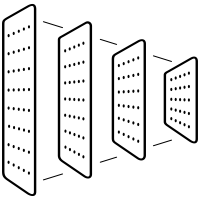
\includegraphics[width=2cm]{image/Resim45.png} % Resmin dosya adı ve boyutu
\end{textblock*}
\subsubsection{Havuzlama (Küçültme) Katmanı (Pooling Layer)}
Bu katman, ağın boyutunu küçültmek ve hesaplama yükünü azaltmak için kullanılır. Ayrıca, özelliklerin translasyon ve ölçek değişikliklerine karşı daha dayanıklı hale gelmesine yardımcı olabilir.

\subsubsection{Düzleştirme Katmanı (Flattening Layer)}
Bu katman, evrişimli ve havuzlama katmanlarının çıkışını düzleştirir ve tek boyutlu bir vektöre dönüştürür. Bu, klasik bir sinir ağı için veri hazırlamak için gereklidir.
\subsubsection{Tam Bağlantılı Katman (Fully-Connected Layer)}
 Bu katman, ağın sınıflandırma yapmasını sağlar. Tüm özellikler birbirine bağlanır ve çıktı katmanına yönlendirilir. Standart sinir ağı yapısıdır ve sınıflandırma veya regresyon gibi görevler için kullanılır.\\[5pt]

\noindent Bu katmanlar, bir evrişimli sinir ağının (CNN) temel bileşenlerini oluşturur. Girdi verisinden başlayarak, her katman özelliklerin daha karmaşık düzeylerini öğrenir ve sonunda istenen çıktıya ulaşır.\\[5pt]

\begin{figure}[h]
  \centering
  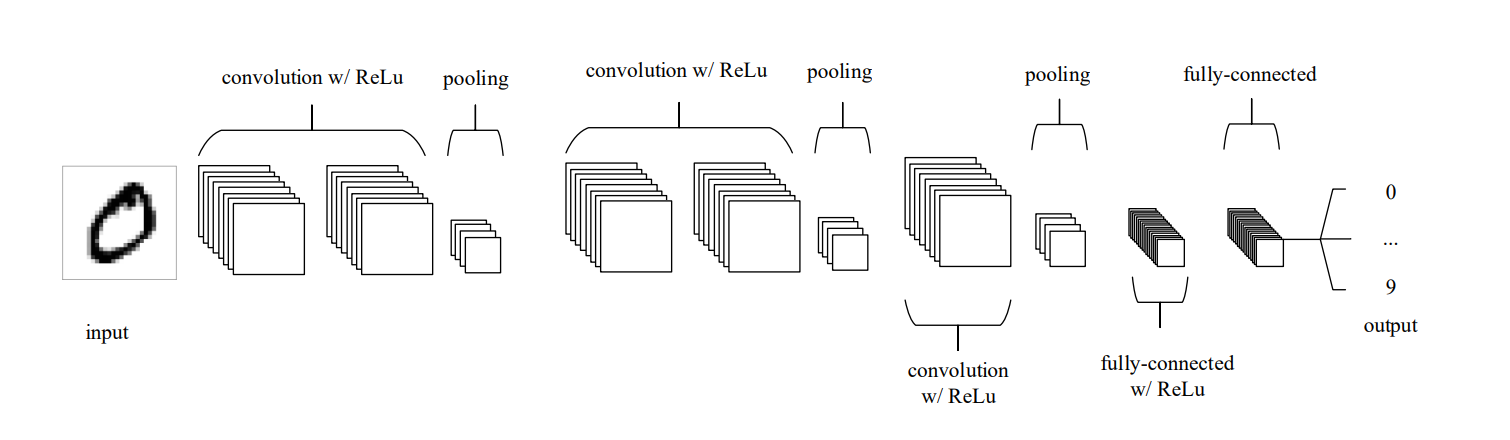
\includegraphics[width=1.1\textwidth]{image/Resim57.PNG} % Resim dosyasının adını ve uzantısını belirtin
\caption{
Beş katmandan oluşan basit bir Evrişimli Sinir Ağı (CNN) mimarisi.\cite{o2015introduction}}
  \label{fig:cnn}  
\end{figure}





\newpage
\begin{textblock*}{5cm}(17cm,1cm) % (17cm, -2cm) koordinatlarına bir text block oluşturulur
    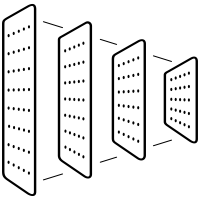
\includegraphics[width=2cm]{image/Resim45.png} % Resmin dosya adı ve boyutu
\end{textblock*}

\subsection{Trafik İşaretleri Sınıflandırılması İçin Evrişimsel Sinir Ağları Kullanımı}
Bu çalışmada, trafik işareti panellerini algılayıp sınıflandıran otomatik bir sistem geliştirdim. Programlama araçları olarak, alanda en çok kullanılan Python, TensorFlow ve Keras'ı kullandım.Bu çalışma, otonom sürüş sistemlerinin güvenilirliğini ve etkinliğini artırmak için önemli bir adımdır. Derin öğrenme ve görüntü işleme tekniklerinin birleşimi, trafik işaretlerinin doğru bir şekilde tanınması ve sınıflandırılmasında etkili bir araç sağlar, bu da güvenliği artırır ve sürüş deneyimini geliştirir.\\[3pt]
\begin{figure}[h]
  \centering
  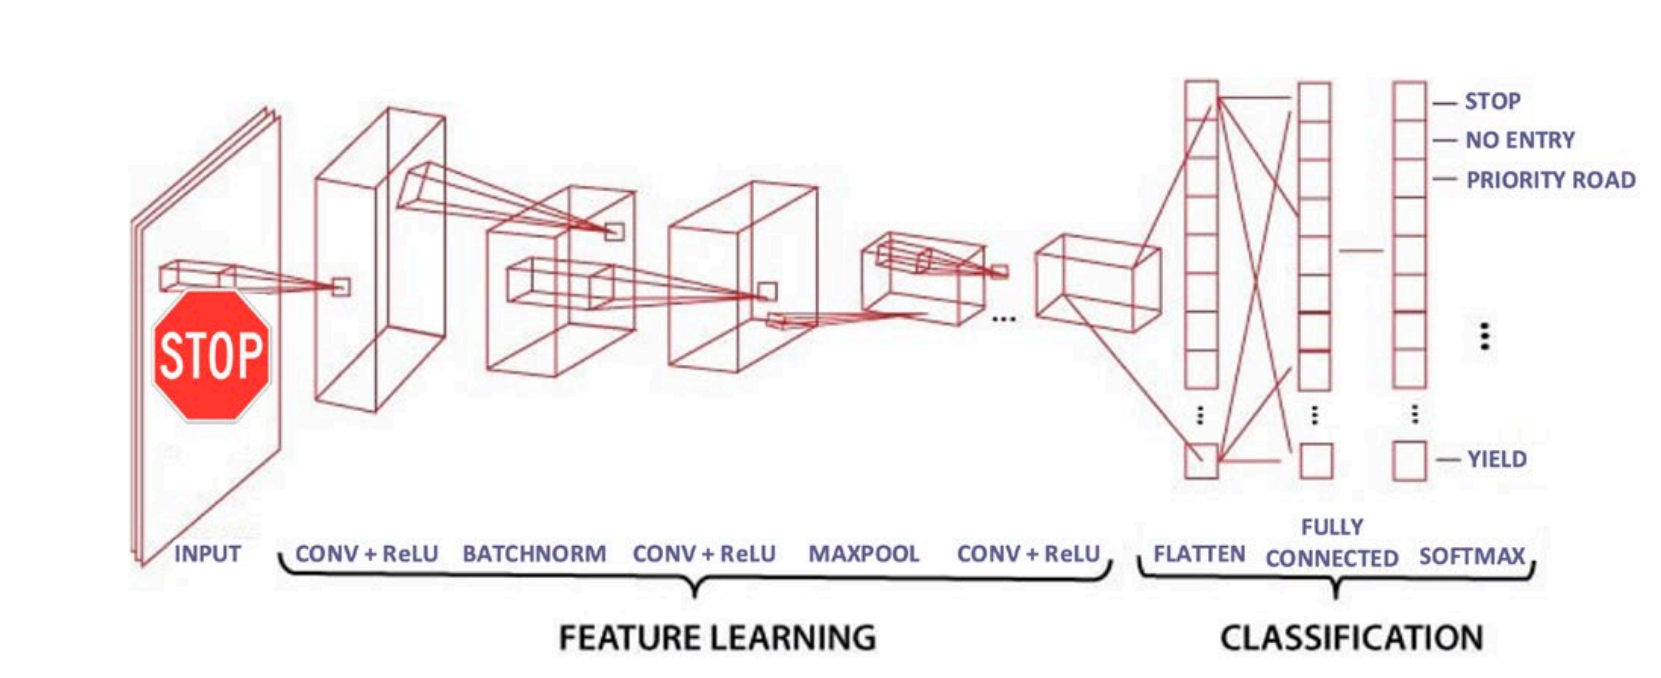
\includegraphics[width=1\textwidth]{image/Resim52.PNG} % Resim dosyasının adını ve uzantısını belirtin
\caption{Uygulamalı sınıflandırma katmanı yapısı.\cite{ferencz2024neural}}
  \label{fig:cnnmimari}  
\end{figure}


\begin{table}[htbp]
\centering
\caption{Ağ Katmanları ve Çıkış Şekilleri}
\begin{tabular}{|l|l|l|}
\hline
\textbf{Katman (Tür)}           & \textbf{Çıkış Şekli} & \textbf{Parametre Sayısı} \\ \hline
conv2d (Conv2D)                 & (None, 28, 28, 60)   & 1,560                     \\ \hline
conv2d\_1 (Conv2D)              & (None, 24, 24, 60)   & 90,060                    \\ \hline
max\_pooling2d (MaxPooling2D)   & (None, 12, 12, 60)   & 0                         \\ \hline
conv2d\_2 (Conv2D)              & (None, 10, 10, 30)   & 16,230                    \\ \hline
conv2d\_3 (Conv2D)              & (None, 8, 8, 30)     & 8,130                     \\ \hline
max\_pooling2d\_1 (MaxPooling2D) & (None, 4, 4, 30)     & 0                         \\ \hline
dropout (Dropout)               & (None, 4, 4, 30)     & 0                         \\ \hline
flatten (Flatten)               & (None, 480)          & 0                         \\ \hline
dense (Dense)                   & (None, 500)          & 240,500                   \\ \hline
dropout\_1 (Dropout)             & (None, 500)          & 0                         \\ \hline
dense\_1 (Dense)                 & (None, 43)           & 21,543                    \\ \hline
\end{tabular}
\label{tab:network_layers}
\end{table}
\newpage
\begin{textblock*}{5cm}(17cm,1cm) % (17cm, -2cm) koordinatlarına bir text block oluşturulur
    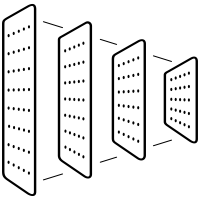
\includegraphics[width=2cm]{image/Resim45.png} % Resmin dosya adı ve boyutu
\end{textblock*}


\subsubsection{Veri Kümesi}
Projemde Alman Trafik İşareti Tanıma Karşılaştırması (GTSRB)\cite{ElectronicResearchDataArchive} veri setini kullandım.Bu veri seti, her bir görüntünün ilgili sınıfa göre etiketlendiği, Alman yollarından alınan trafik işaretlerinin görüntülerinden oluşur.Veri setindeki her görüntü 32 x 32 piksel çözünürlüğe sahiptir ve üç renk kanalıyla RGB formatında temsil edilir.Veri seti, trafik işaretlerinin tasarımına veya anlamına bağlı olarak toplam 43 farklı sınıf veya etiketten oluşmaktadır.Eğitim seti, her biri ilgili etiketle ilişkilendirilmiş 34.799 görüntüden oluşur.Doğrulama seti, ilgili etiketleriyle birlikte 4.410 resim içerir.Son olarak test seti, her biri ilgili sınıfla etiketlenmiş 12.630 görüntüden oluşur.\\[5pt]

\begin{figure}[h]
  \centering
  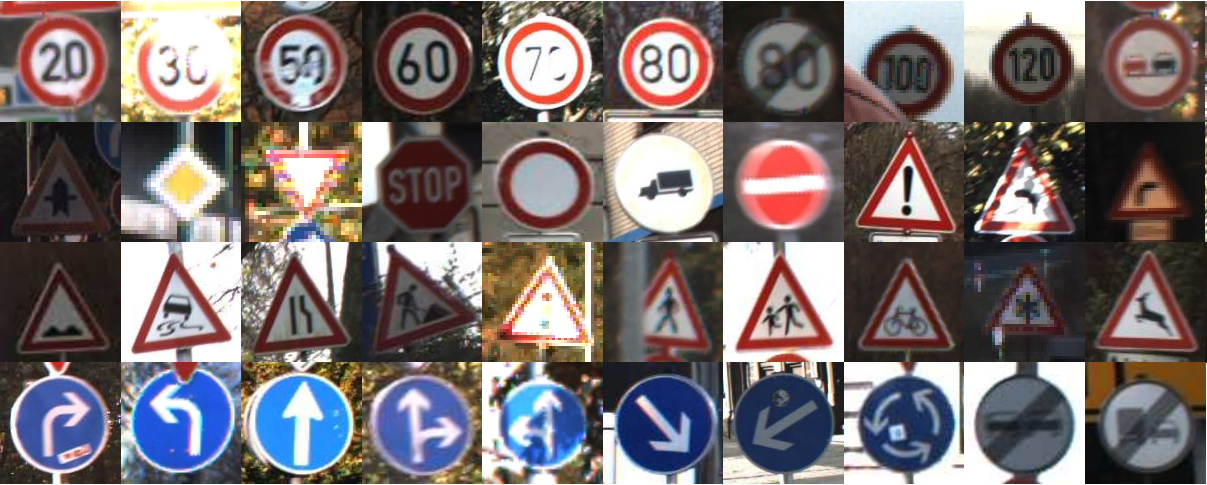
\includegraphics[width=1\textwidth]{image/Resim44.PNG} % Resim dosyasının adını ve uzantısını belirtin
\caption{Veri kümesinden görüntüler.\cite{stallkamp2011german}}
  \label{fig:cnnmimari}  
\end{figure}


\begin{figure}[h]
  \centering
  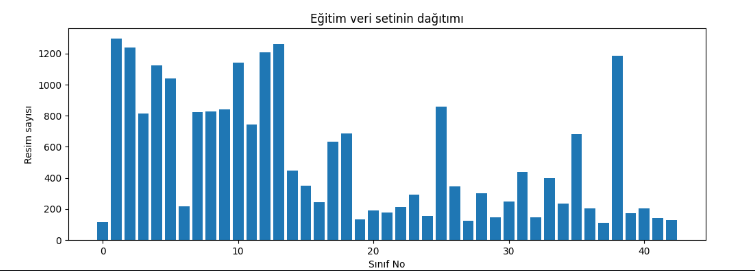
\includegraphics[width=1.1\textwidth]{image/Resim48.PNG} % Resim dosyasının adını ve uzantısını belirtin
\caption{Eğitim veri seti dağılım grafiği}
  \label{fig:cnnmimari}  
\end{figure}
\newpage
\begin{textblock*}{5cm}(17cm,1cm) % (17cm, -2cm) koordinatlarına bir text block oluşturulur
    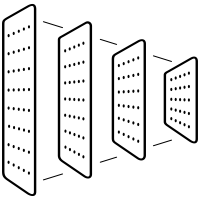
\includegraphics[width=2cm]{image/Resim45.png} % Resmin dosya adı ve boyutu
\end{textblock*}
\subsubsection{Sonuçlar}
\noindent Modelin test seti üzerinde elde ettiği sonuçlar, trafik işaretlerini doğru bir şekilde sınıflandırabildiğini göstermektedir. Ancak, gerçek dünya koşullarında performansın değerlendirilmesi için daha fazla test yapılması gerekmektedir.
\begin{figure}[htbp]
    \centering
    \begin{minipage}{0.45\textwidth}
        \centering
        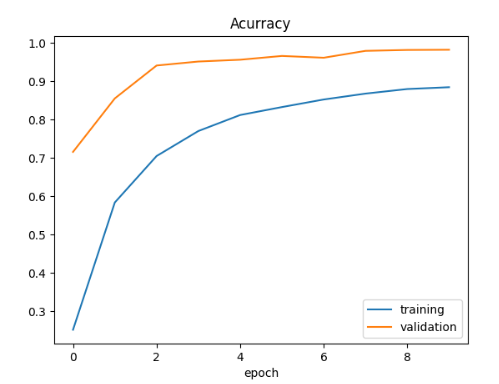
\includegraphics[
        width=7cm,
        height=7cm,
        keepaspectratio,]{image/Resim46.png}
    \end{minipage}
    \hfill
    \begin{minipage}{0.45\textwidth}
        \centering
        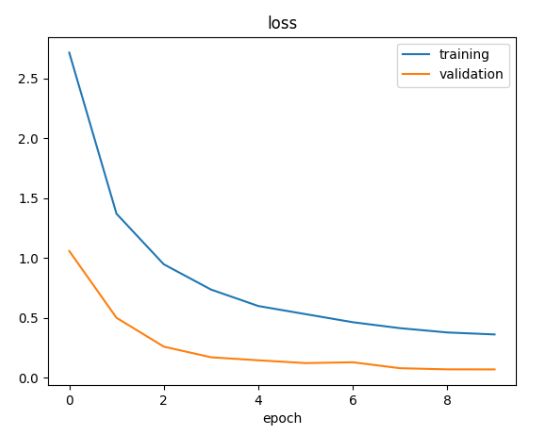
\includegraphics[
        width=7cm,
        height=7cm,
        keepaspectratio,]{image/Resim47.png}
    \end{minipage}
\end{figure}


\begin{table}[htbp]
\centering
\caption{Test Sonuçları}
\begin{tabular}{|l|l|}
\hline
\textbf{Test Skoru} & 0.06186366081237793 \\ \hline
\textbf{Test Doğruluğu} & 0.9844827651977539 \\ \hline
\end{tabular}
\label{tab:test_results}
\end{table}
\noindent \\[5pt] Bu tablo [\ref{tab:test_results}], test sonuçlarını özetlemektedir. "Test Skoru" sütunu, modelin test veri kümesi üzerinde elde ettiği ortalama kayıp (loss) değerini gösterirken, "Test Doğruluğu" sütunu ise modelin test veri kümesi üzerindeki doğruluk oranını temsil eder. Örneğin, "Test Doğruluğu" sütunu 0.9844 değerini alıyor, yani model test veri kümesindeki örneklerin yaklaşık 98.45'ini doğru bir şekilde sınıflandırıyor.
\newpage
\begin{textblock*}{5cm}(17cm,1cm) % (17cm, -2cm) koordinatlarına bir text block oluşturulur
    \includegraphics[width=2cm]{image/Resim45.png} % Resmin dosya adı ve boyutu
\end{textblock*}
\subsubsection{Projeden görüntüler}
\begin{figure}[h]
    \centering
    \begin{subfigure}{0.5\textwidth}
        \centering
        \includegraphics[width=1\linewidth]{image/Resim50.PNG}
        \caption{German Stop Sign}
        \label{fig:resim1}
    \end{subfigure}%
    \begin{subfigure}{0.5\textwidth}
        \centering
        \includegraphics[width=1.1\linewidth]{image/Resim51.PNG}
        \caption{German Wild Animals Crossing Sign}
        \label{fig:resim2}
    \end{subfigure}
    \caption{Farklı trafik işaretleri üzerinde farklı denemeler yapılmıştır.}
    \label{fig:iki_resim}
\end{figure}

\section{Sonuç}
Bu projelerde, otonom araç sistemlerinde kullanılan çeşitli teknolojileri kapsadım. Temel amacım, otonom araçların güvenli ve etkili bir şekilde hareket etmelerini sağlamak için kullanılan teknikleri anlamak ve uygulamaktı.\\[2pt]
İlk olarak, aracın hareket yolunu belirlemek için şerit çizgilerini tespit etmek için OpenCV kütüphanesini kullandım. Bu adım, aracın konumunu belirlemede kritik bir rol oynuyor.\\[2pt]
Ardından, Lojistik Regresyon ile Sınıflandırma ve Yapay Sinir Ağı ile Sınıflandırma ve Tahmin projeleri gibi makine öğrenimi yöntemlerini kullanarak, araçların çevresini algılamalarını ve bu bilgileri temel alarak çeşitli sınıflandırma ve tahmin işlemlerini gerçekleştirmelerini sağladım. Bu adımlar, araçların çevrelerindeki nesneleri tanımalarını ve hareketlerini buna göre ayarlamalarını sağlar.\\[2pt]
Son olarak, trafik işaretlerinin tanınması ve sınıflandırılması için Evrişimsel Sinir Ağları (CNN) kullanarak, araçların trafik kurallarını algılamalarını ve uygun şekilde tepki vermelerini sağladım. Bu, otonom araçların trafikte diğer araçlarla etkileşimini optimize etmek için önemli bir adımdır.\\[2pt]
Bu projelerin sonuçları, otonom araç teknolojilerinin gelişimine katkıda bulunmak için temel bir adım olarak değerlendirilebilir. Elde ettiğim sonuçlar, otonom araçların çevrelerini algılamak ve çeşitli görevleri yerine getirmek için kullanılan teknolojilerin etkinliğini ve potansiyelini gösteriyor. Gelecekte, bu çalışmaların temelini oluşturarak, otonom araçların daha güvenli, verimli ve yaygın olarak kullanılabilir hale gelmesine katkıda bulunmayı umuyorum.
\newpage
\subsection{Gelecekteki çalışmalar}
Gelecekte, Udacity otonom sürüş simülasyonu üzerinde uyguladığım bilgi ve deneyimleri kullanarak bir otonom araç sistemi geliştirmeyi planlıyorum. Bu simülasyon, gerçek dünya koşullarını taklit ederek, otonom araçların performansını test etmek için ideal bir ortam sunuyor. Bu projede, mevcut algoritmaları simülasyon ortamına entegre etmek ve daha karmaşık algoritmalar geliştirmek için çalışacağım. Amacım, güvenilir ve etkili bir otonom sürüş deneyimi sağlayacak bir sistem oluşturmaktır.











\bibliographystyle{ieeetr}
\bibliography{referans}
\end{document}
